\subsection{Motivation}

\begin{frame}{Scenario}

    \vspace{1em}
    \begin{columns}[onlytextwidth]
        \begin{column}{0.65\textwidth}
            \begin{figure}
                \includegraphics<1>[width=\textwidth]{figures/scene1.png}
                \includegraphics<2>[width=\textwidth]{figures/scene2.png}
                \includegraphics<3>[width=\textwidth]{figures/scene3.png}
                \includegraphics<4>[width=\textwidth]{figures/scene4.png}
                \includegraphics<5>[width=\textwidth]{figures/scene5.png}
            \end{figure}
        \end{column}
        \begin{column}{0.34\textwidth}
            \textbf{Sound}
            \begin{itemize}
                \item<1-> produced by \alert{sources}
                \item<2-> recorded by \alert{microphones}
                \item<3-> corrupted by \alert{noise}
                \only<4>{\item propagates in the \alert{space}}
                \only<5->{\item propagates in the \alert{room}
                          \\$\hookrightarrow$ \alert{reverberation}}
            \end{itemize}
        \end{column}
    \end{columns}

    \vfill
    \textcolor{gray}{Attention: artificial sound vs \textbf{(natural) microphone recordings}}

\end{frame}

\begin{frame}[t]{Echo-aware signal processing for \alert{audio scene analysis}}

    \begin{columns}
        \begin{column}[t]{0.3\textwidth}
            \centering
            \alert{Semantic} information

            \vspace*{0.5em}
            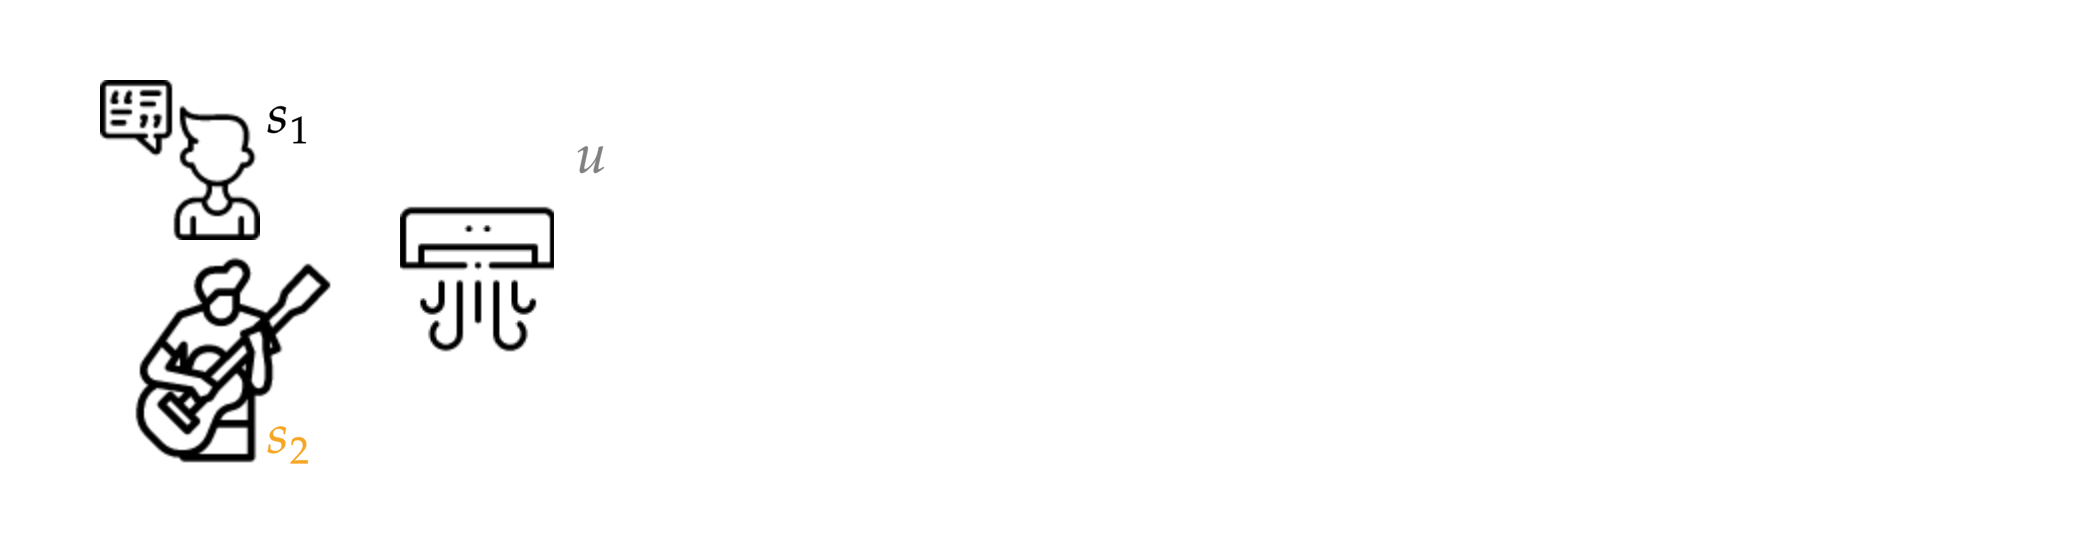
\includegraphics[trim={0 0 170em 0},clip,width=\textwidth]{figures/semantic.png}
            about source nature and semantic content
        \end{column}
        \begin{column}[t]{0.3\textwidth}
            \centering
            \alert{Spatial} information

            \vspace*{0.5em}
            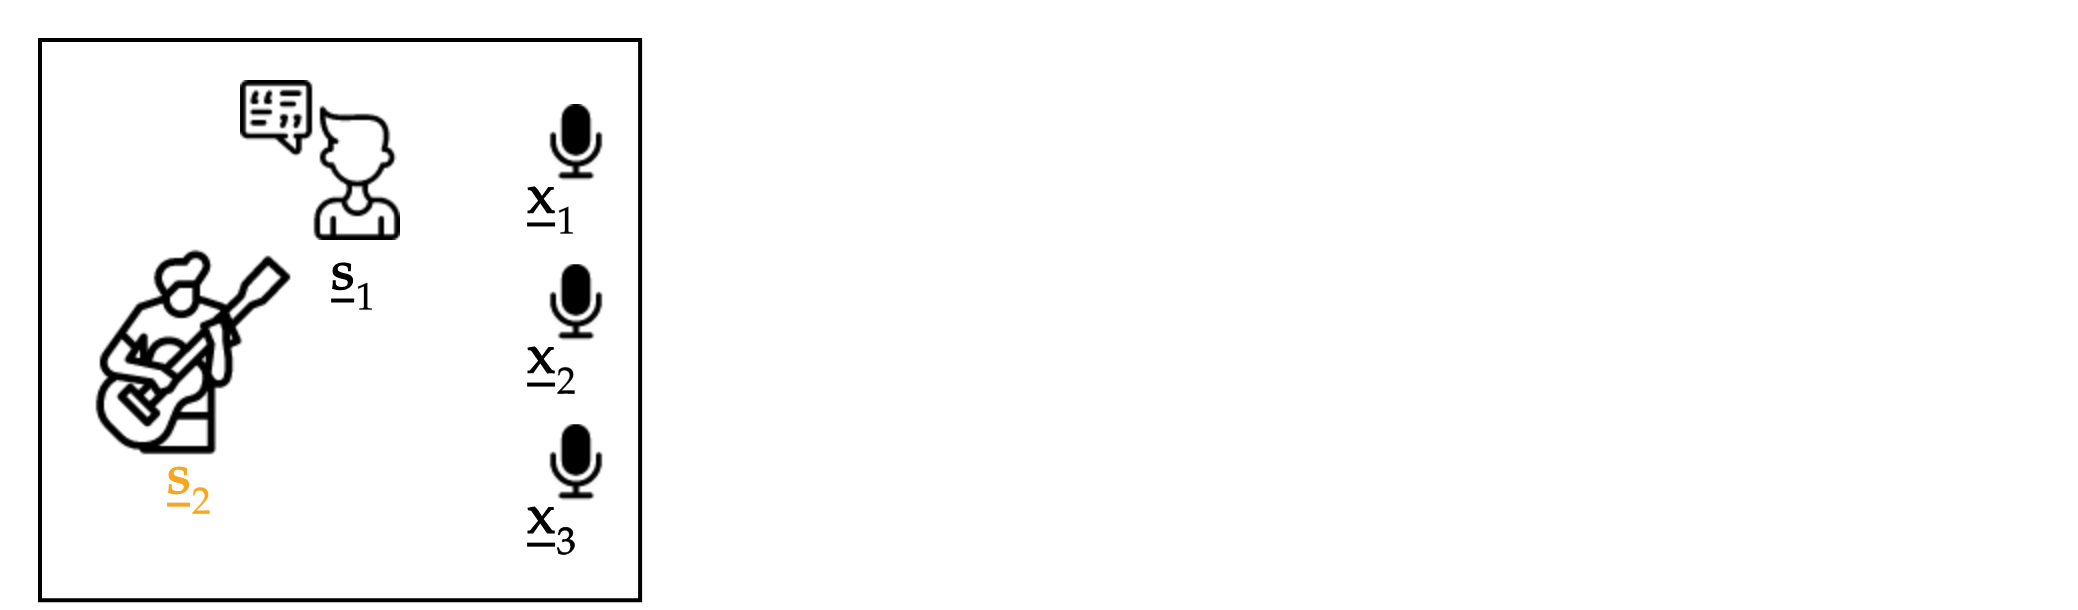
\includegraphics[trim={0 0 170em 0},clip,width=\textwidth]{figures/spatial.png}
            about source position and room geometry
        \end{column}
        \begin{column}[t]{0.3\textwidth}
            \centering
            \alert{Temporal} information

            \vspace*{0.5em}
            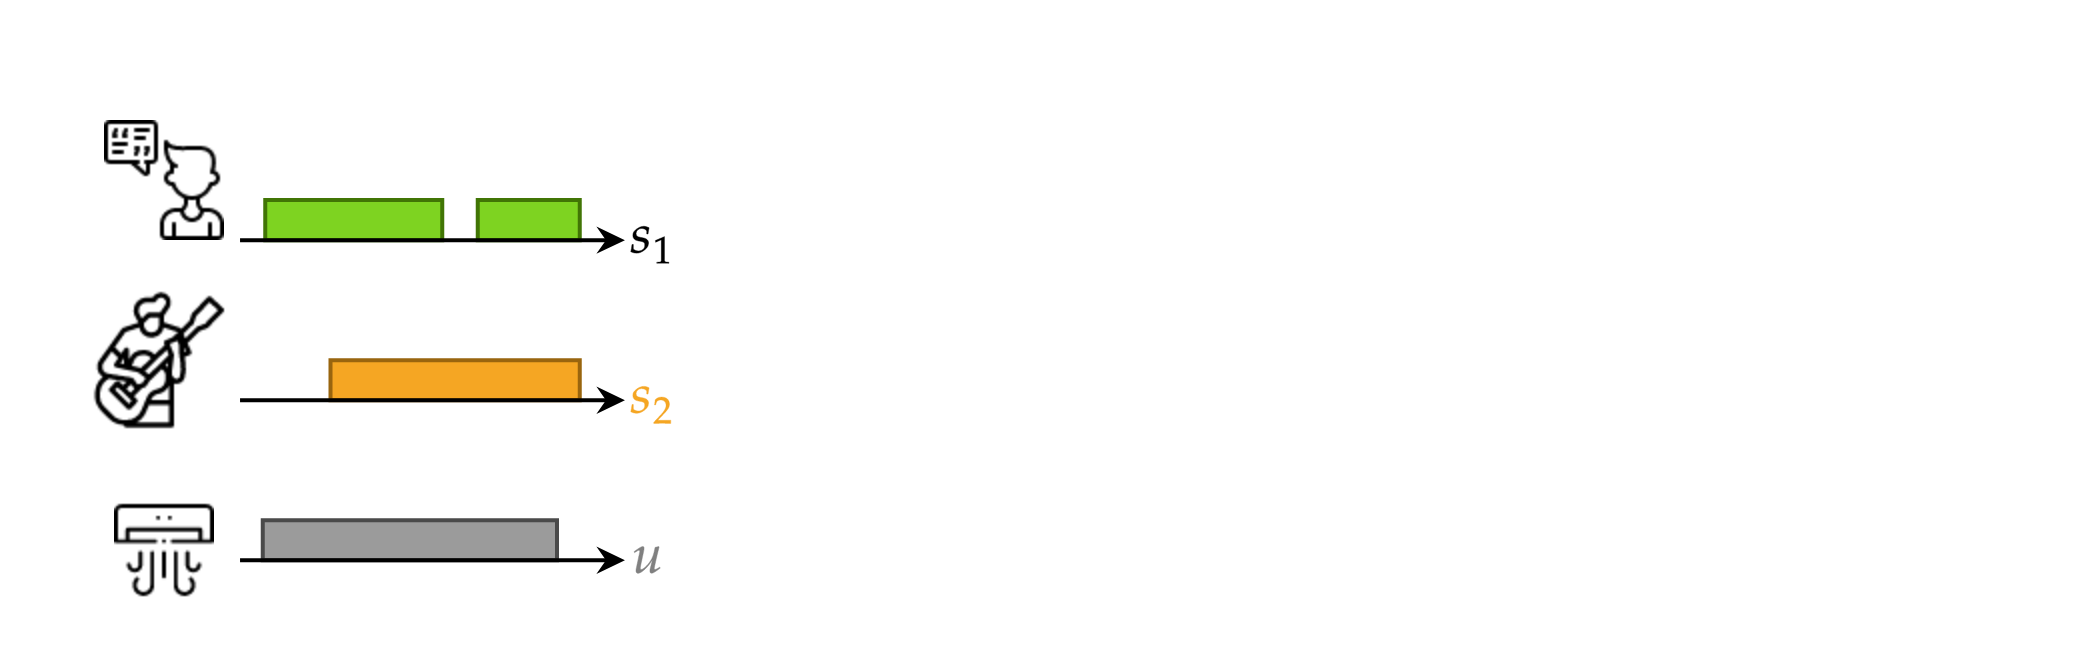
\includegraphics[trim={0 0 170em 0},clip,width=\textwidth]{figures/temporal.png}
            about events activity
        \end{column}
    \end{columns}

    \vfill
    \begin{mydefblock}{Audio Scene Analysis}
        Extraction and organization of all the information in the sound
    \end{mydefblock}

    \vfill
    \begin{center}
        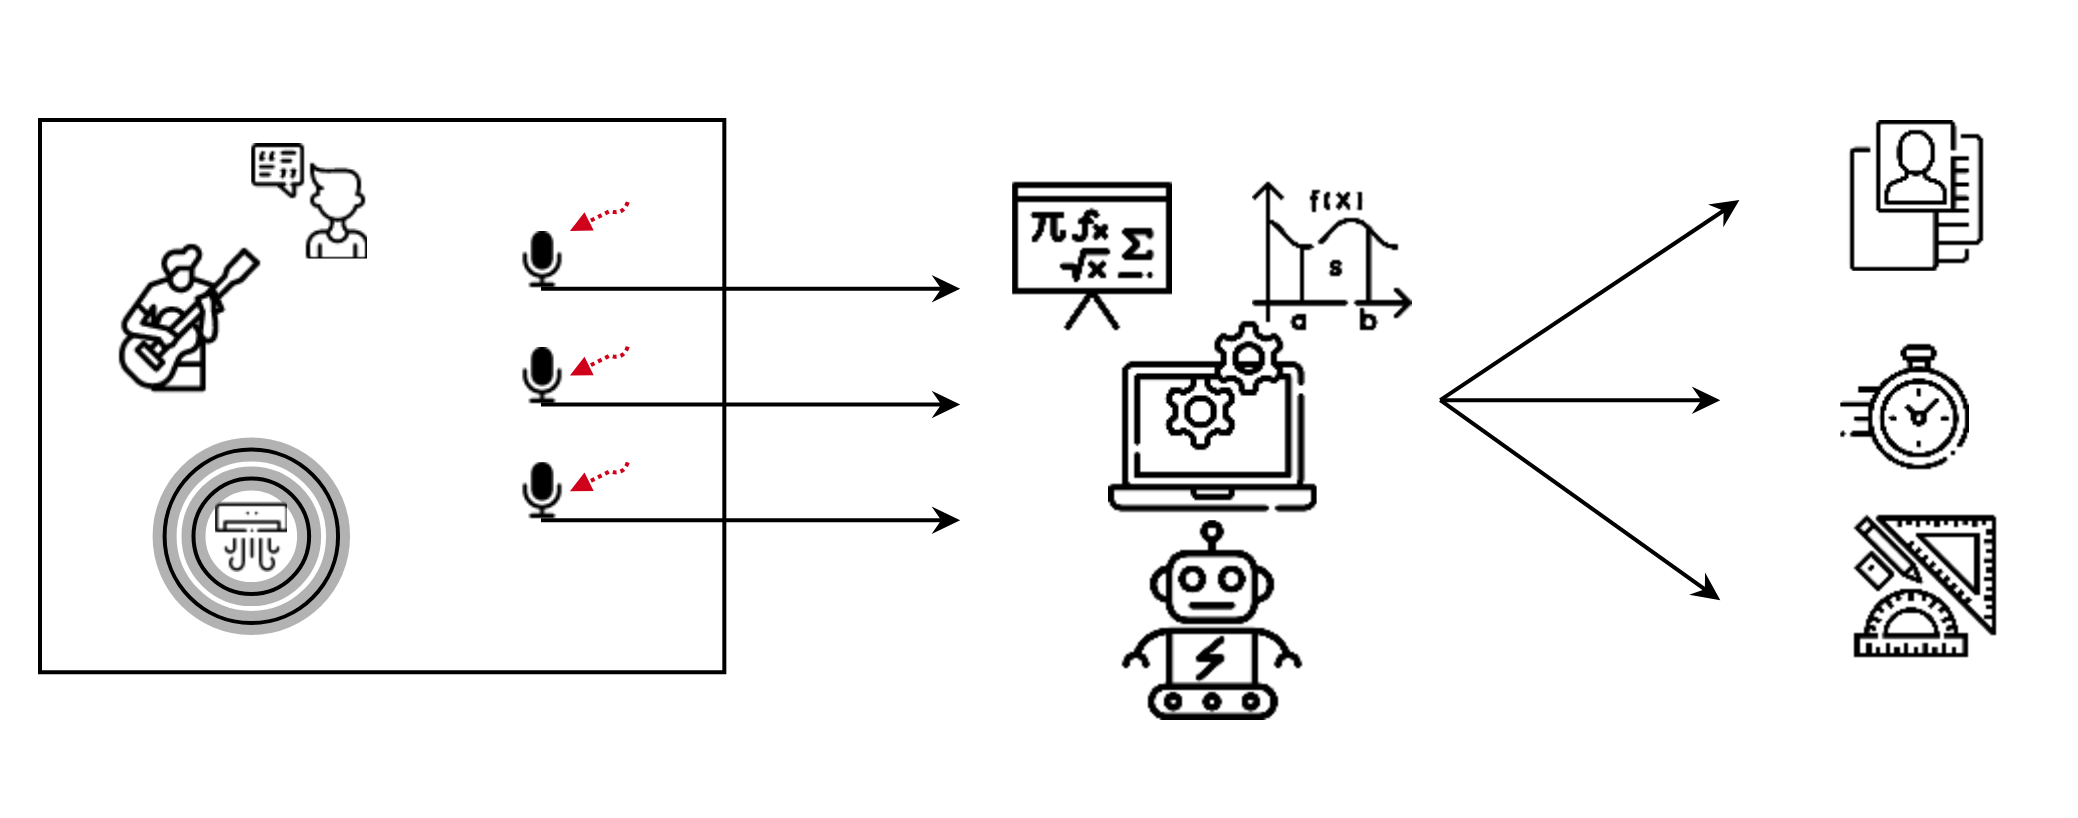
\includegraphics[width=0.8\textwidth]{figures/scene_analysis.png}
    \end{center}

    Animals do it, humans do it,
    \\\hfill\textcolor{myred}{\textbf{can computer do it?}}

\end{frame}

\begin{frame}[t]{Echo-aware \alert{signal processing for audio scene analysis}}

    \begin{mydefblock}{Signal Processing}
        Mathematical models, frameworks and tools to tackle and solve such problems
    \end{mydefblock}

    \vfill
    \begin{columns}[onlytextwidth]
        \begin{column}{0.55\textwidth}
            \begin{figure}
                \includegraphics[width=\textwidth]{example-image-a}
            \end{figure}
        \end{column}\hfill
        \begin{column}{0.42\textwidth}
            \small
            Some problems
            \begin{itemize}
                \item Speaker Verification\tikzmark{top1}\tikzmark{bot1}
                \item Sound Source Separation \tikzmark{top2}
                \item Speech Enhancement
                \item Automatic Speech Recognition\hspace{0.5em}\tikzmark{right1}\tikzmark{bot2}
                \item Sound Source Localization  \tikzmark{top3}
                \item Room Geometry Estimation   \tikzmark{bot3}
                \item Voice Activity Detection   \tikzmark{top4}
                \item Diarization                \tikzmark{bot4}
                \item RT$_{60}$ estimation       \tikzmark{top5}
                \item Wall Absorption Estimation \tikzmark{bot5}
                \item \textit{and many many other}
            \end{itemize}

            \begin{tikzpicture}[overlay, remember picture]
                \node[anchor=base] (a) at (pic cs:top1) {\vphantom{h}}; % push the mark to the top of the line (ie including ascenders)
                \node[anchor=base] (b) at (pic cs:bot1) {\vphantom{g}}; % push the mark to the bottom of the line (ie including descenders)
                \draw [decoration={brace,amplitude=0.5em},decorate,thick,gray]
                 (a.north -| {pic cs:right1}) -- node[right,inner sep=1em] {Who?} (b.south -| {pic cs:right1});
            \end{tikzpicture}
            \begin{tikzpicture}[overlay, remember picture]
                \node[anchor=base] (a) at (pic cs:top2) {\vphantom{h}}; % push the mark to the top of the line (ie including ascenders)
                \node[anchor=base] (b) at (pic cs:bot2) {\vphantom{g}}; % push the mark to the bottom of the line (ie including descenders)
                \draw [decoration={brace,amplitude=0.5em},decorate,thick,gray]
                 (a.north -| {pic cs:right1}) -- node[right,inner sep=1em] {What?} (b.south -| {pic cs:right1});
            \end{tikzpicture}
            \begin{tikzpicture}[overlay, remember picture]
                \node[anchor=base] (a) at (pic cs:top3) {\vphantom{h}}; % push the mark to the top of the line (ie including ascenders)
                \node[anchor=base] (b) at (pic cs:bot3) {\vphantom{g}}; % push the mark to the bottom of the line (ie including descenders)
                \draw [decoration={brace,amplitude=0.5em},decorate,thick,gray]
                 (a.north -| {pic cs:right1}) -- node[right,inner sep=1em] {Where?} (b.south -| {pic cs:right1});
            \end{tikzpicture}
            \begin{tikzpicture}[overlay, remember picture]
                \node[anchor=base] (a) at (pic cs:top4) {\vphantom{h}}; % push the mark to the top of the line (ie including ascenders)
                \node[anchor=base] (b) at (pic cs:bot4) {\vphantom{g}}; % push the mark to the bottom of the line (ie including descenders)
                \draw [decoration={brace,amplitude=0.5em},decorate,thick,gray]
                 (a.north -| {pic cs:right1}) -- node[right,inner sep=1em] {When?} (b.south -| {pic cs:right1});
            \end{tikzpicture}
            \begin{tikzpicture}[overlay, remember picture]
                \node[anchor=base] (a) at (pic cs:top5) {\vphantom{h}}; % push the mark to the top of the line (ie including ascenders)
                \node[anchor=base] (b) at (pic cs:bot5) {\vphantom{g}}; % push the mark to the bottom of the line (ie including descenders)
                \draw [decoration={brace,amplitude=0.5em},decorate,thick,gray]
                 (a.north -| {pic cs:right1}) -- node[right,inner sep=1em] {How?} (b.south -| {pic cs:right1});
            \end{tikzpicture}
        \end{column}
    \end{columns}
    % \pause
    % Also known as auditory scene analysis or computer auditory scene analysis.
    % \\Inverse and Forward problems
    % \\Blind and Informed problems

    \vfill
    \begin{block}{Everything is connected}
        HOW  $\rightarrow$ WHERE $\rightarrow$ WHEN $\rightarrow$ WHAT
    \end{block}

\end{frame}


% \begin{frame}{Echo-aware \alert{signal processing} for audio scene analysis}

%     \vfill
%     \begin{block}{Signal Model}
%         \begin{columns}
%             \begin{column}{0.45\textwidth}
%                 \centering
%                 \includegraphics[width=0.5\textwidth]{example-image-a}
%             \end{column}
%             \begin{column}{0.58\textwidth}
%                 \begin{itemize}
%                     \item produced by sources
%                     \item propagates in the room
%                     \item corrupted by noise
%                     \item recorded by microphone
%                 \end{itemize}
%             \end{column}
%         \end{columns}
%     \end{block}

% \end{frame}

\begin{frame}[t]{\alert{Echo-aware signal processing for audio scene analysis}}

    \begin{mydefblock}{Acoustic Echoes}
        \begin{itemize}
            \item Elements of the sound propagation
            \item Sound reflection standing out for time and strength w.r.t. to the total reverberation
            \item repetition of the source sound but later
            \item both outdoor and indoor
        \end{itemize}
    \end{mydefblock}

    \vfill
    \begin{block}{}
        Audio signal processing w.r.t. sound propagation~\cite{chen1993time}
        \begin{itemize}
            \item ignore it
            \item assume it free-field
            \item model it entirely
            \item model as few reflection $\rightarrow$ echo-aware processing
        \end{itemize}

    \end{block}

    % \vfill
    % \begin{block}{Echo-aware processing}
    % \end{block}

    % \begin{columns}[T,onlytextwidth]
    %     \begin{column}{0.3\textwidth}
    %         \alert{Free-field} processing
    %         \\{\small(only direct path)}
    %     \end{column}\hfill
    %     \begin{column}{0.3\textwidth}
    %         \alert{Echo} processing
    %         \\{\small(only specular reflection)}
    %     \end{column}\hfill
    %     \begin{column}{0.3\textwidth}
    %         \alert{Reverberant} processing
    %         \\{\small(entire sound field)}
    %     \end{column}
    % \end{columns}%

    % \vfill
    % \begin{columns}[T,onlytextwidth]
    %     \begin{column}{0.3\textwidth}
    %         \small
    %         \begin{itemize}
    %             \item[\cmark] \textcolor{mygreen}{``simple'' processing} %closed-from formulas %fully deterministic
    %             \item[\cmark] \textcolor{mygreen}{``short'' processing} % STFT, no latency
    %             \item[\xmark] \textcolor{myred}{Reflection are interferences}
    %             \item[\xmark] \textcolor{myred}{Neglect most of the sound energy}
    %             \item[\xmark] \textcolor{myred}{incoherence $\implies$ distortion}
    %         \end{itemize}
    %     \end{column}\hfill
    %     \begin{column}{0.3\textwidth}
    %         \small
    %         \begin{itemize}
    %             \item short processing %  echoes $\rightleftarrows$ positions
    %             \item simple processing
    %             \item reflection are integrated,
    %             \\late reverberation can considered
    %             \item reflection are difficult to estimate
    %             \item reflection need to be correctly estimated
    %         \end{itemize}
    %     \end{column}\hfill
    %     \begin{column}{0.3\textwidth}
    %         \small
    %         \begin{itemize}
    %             % fully deterministic and stochastic processing
    %             \item difficult processing %estimation is extremely difficult, more parameters to estimate
    %             \item long precessing
    %             \item Reflection perfectly integrated
    %         \end{itemize}
    %     \end{column}
    % \end{columns}

    %     \\Anechoic processing
    %     \begin{itemize}
    %         \item short processing
    %         \item[\cmark] sound field tends to be diffuse
    %         \item[\xmark] sound reflection as interferences
    %         \\neglect most of the sound energy
    %         \\ignore the correlation between the direct sound and its reflection and consequently may result in a distorted output
    %         \item[\xmark] coherent processing becomes impossible
    %     \end{itemize}
    %     Echo-processing
    %     \begin{itemize}
    %         \item Middle processing
    %         perceive coming from all directions~\cite{daldegan1988}
    %     \end{itemize}
    %     Reverberant processing
    %     \begin{itemize}
    %         \item Long processing
    %         \item[\cmark] narrowband approximation is valid
    %         \item[\cmark] sound field is described by full RIRs
    %         \item[\cmark] all reflection can be \alert{coherently} processed
    %         \item[\xmark] long frames impose lantency
    %     \end{itemize}
    % \end{block}

\end{frame}

\subsection{Outline}

\begin{frame}[t]{Thesis goal and contribution}

    \vfill
    \begin{columns}[onlytextwidth]
        \begin{column}[T]{0.3\linewidth}
            \centering
            \textbf{Audio Scene Analysis}
            \\\downarrow
            \\context and problems
        \end{column}\hfill
        \begin{column}[T]{0.3\linewidth}
            \centering
            \textbf{Signal Processing}
            \\\downarrow
            \\models and frameworks
        \end{column}\hfill
        \begin{column}[T]{0.3\linewidth}
            \centering
            \textbf{Acoustic Echoes}
            \\\downarrow
            \\better processing
        \end{column}\hfill
    \end{columns}

    \vfill
    \begin{mydefblock}{Thesis objective}
        \begin{enumerate}
        \item provide new methodologies and data to process and estimate acoustic echoes
        \item Turning echoes into friends \cite{Riberio}
        \\extend previous classical methods for audio scene analysis
        \end{enumerate}
    \end{mydefblock}

    \vfill
    \begin{block}{contribution}
        Estimation
        \begin{itemize}
            \item Knowledge-based echo estimation, aka \blaster
            \item Learning-based echo estimation, aka \lantern
        \end{itemize}
        Application
        \begin{itemize}
            \item Echo-aware Source Separation, aka \separake
            \item Echo-aware Source Localization, aka \mirage
            \item Echo-aware Speech Enhancement
            \item Echo-aware Room Geometry Estimation
        \end{itemize}
        Data
        \begin{itemize}
            \item a Echo-aware database, aka \dechorate
        \end{itemize}
    \end{block}

\end{frame}

% change color of Beamer subsection
% https://tex.stackexchange.com/questions/356237/changing-text-color-in-subsection-in-tableofcontents-in-beamer
\begin{frame}[standout]{1D Outline}
    \begin{columns}
        \begin{column}{0.35\textwidth}
            Echo-aware signal processing
            \\for audio scene analysis
        \end{column}
        \begin{column}{0.05\textwidth}
        \end{column}
        \begin{column}{0.6\textwidth}
            {
                \setbeamercolor{part in toc}{fg=gray}
                \setbeamercolor{section in toc}{fg=gray}
                \setbeamercolor{subsection in toc}{fg=white}
                \tableofcontents
            }
        \end{column}
    \end{columns}
\end{frame}